% TODO Skrive mer om LSP (diagram)

\documentclass[12pt]{article}

\setlength\parindent{0pt}

\usepackage[english]{babel}
\usepackage{graphicx}
\usepackage{amsmath}
\usepackage{tikz}
\usepackage{hyperref}
\usepackage{graphicx}
\usepackage[a4paper, total={}]{geometry}
\setlength{\headsep}{5pt}
\setlength{\parskip}{1em}
\usepackage{listings}

\definecolor{pblue}{rgb}{0.2,0.2,0.7}
% \definecolor{pgreen}{rgb}{0,0.5,0}
\definecolor{pred}{rgb}{0.7,0.2,0.2}
\definecolor{pgrey}{rgb}{0.46,0.45,0.48}

\lstset{
	backgroundcolor = \color{lightgray},
	language=Bash,
	showstringspaces=false,
	columns=flexible,
	basicstyle={\small\ttfamily},
	numbers=none,
	numberstyle=\tiny\color{gray},
	keywordstyle=\color{blue},
	commentstyle=\color{dkgreen},
	stringstyle=\color{mauve},
	breaklines=true,
	breakatwhitespace=true,
	tabsize=3
}

\hbadness=10000

\usetikzlibrary{automata, positioning, arrows}

\tikzset{
	->,
	node distance=3cm,
	initial text=$ $,
}

\title{\vspace{-20px}Real-time management of code clones in an IDE environment}
% Alternative: \title{IDE-agnostic management of code clones }

\author{Jakob Hansen}

\date{\today}

\begin{document}
\maketitle

\newpage

\tableofcontents

\newpage

\section{Introduction}

Refactoring is the process of restructuring code in order to improve the internal behavior
of the code, without changing the external behavior\cite[9]{fowlerrefactoring}.
Refactoring is often done in order to eliminate instances of bad design quality in code,
otherwise known as code smells.

A study conducted by Diego Cedrim et al. has shown that while developers tend to refactor
smelly code, they are rarely successful at eliminating the smells they are
targeting\cite{Rohit_Gheyi_Impact}. A large portion of refactorings even tend to make the
code smellier. Therefore, automated tools to help developers make better refactorings and
perform code analysis is an important field of research.

Duplicated code is a code smell which occurs in practically every large software project.
Code clone analysis has recently become a highly active field of research and many tools have
been developed to detect duplicated code\cite[7]{Inoue_introduction_to_cc}. However, few of
these tools reached and see use in the industry and few have the capability of detecting
more intricate types of duplicated code and managing them in a real-time IDE environment.

This thesis will present a tool and possibly techniques for industry viable clone
detection and management. It will explore the topics of finding and managing clones in
real-time, refactoring-oriented clone management and providing clone management tools in a
modern IDE environment.

\section{Background}

\subsection{Software quality and duplicated code}

Software quality is hard to define. The term ``quality'' is ambiguous and is in the case
of software quality, multidimensional. Quality in itself has been defined as ``conformance
to requirements''\cite[8]{crosby1980quality}. In software, the simplest measure of
``conformance to requirements'' the software can have is a lack of bugs. However, software
quality is often measured in other metrics, including metrics which are not directly
visible in the functionality\cite[29]{MetricsAndModelsInSoftwareQuality}. These metrics
often include maintainability, analyzability and changeability.

All of these stated metrics are affected negatively by duplicated code, code which is more
or less copied to different locations in the software. Multiple studies have consistently
shown that software projects typically have $10-15\%$ duplicated
code\cite{CloningByAccident}. Therefore, research into tools and techniques which can
reduce duplicated code, will be of benefit to almost all software.

As stated, duplicated code damages software quality software projects. Duplicated code can
lead to a plethora of antipatterns, for example shotgun-surgery, and will often lead to an
increase in technical debt for the project\cite[99]{fowlerrefactoring}. The
shotgun-surgery antipattern occurs when a developer wants to implement a change, but needs
to make the same change in many places for the change to take effect. This is a typical
situation which slows down development when a software project contains a lot of
duplicated code.

\subsection{Code clones}

We define a code snippet or code fragment as a piece of software code in a larger software
system. A code clone is then defined as a code snippet which is equal to or similar to
another code snippet. The two code snippets are both code clones, and together they form a
code clone pair.

\subsubsection{The clone relation}
The clone relation defines a relation between code snippets where snippets which are
code clones are related to each other. The clone relation is reflexive and symmetric, but
not always transitive. The transitive property depends on the threshold for similarity when
identifying code clones. Given

$$a \xrightarrow{clone} b \xrightarrow{clone} c$$

where $a,b,c$ are code snippets and $\xrightarrow{clone}$ gives the clone relation, $a$ is
a clone of $b$, but not necessarily similar enough to be a clone of $c$, depending on the
threshold for similarity.

\subsubsection{Code clone types}

Code clones are generally classified into four types\cite{Inoue_introduction_to_cc}. These
types classify code snippets as code clones with an increasing amount of leniency.
Therefore, Type-1 code clones are very similar, while Type-4 clones are not necessarily
similar at all. However, all code clones do still have the same functionality, it is the
syntactic and structural differences which distinguish the types. The set of code clones
classified by a code clone type is also a subset of the next type, meaning all type-1
clones are also type-2 clones, but not vice versa.

The code clone types are defined as follows:

\textbf{Type-1} clones are syntactically identical. The only differences allowed are elements
without meaning, like comments and white-space.

\textbf{Type-2} clones are structurally identical. Possible differences include
identifiers, literals and types.

\textbf{Type-3} clones are required to be structurally similar, but not equal. Differences
include statements which are added, removed or modified. This clone type relies on a
threshold $\theta$ which determines how structurally different snippets can be
to be considered Type-3 clones\cite{Inoue_introduction_to_cc}.

\textbf{Type-4} clones have no requirement for syntactical or structural similarity. Therefore,
the only requirement is having the same functionality.

Type-1 clones are often referred to as ``exact`` clones, while Type-2 and Type-3 clones are
often referred to as ``near-miss`` clones\cite[1]{Zibran_real_time_search}.

\subsubsection{Code clone detection process and techniques}

\textbf{The Code clone detection process} is generally split into (but is not limited to)
a set of steps to identify clones\cite{ComparisonAndEvaluationOfTechniques}. This
process is often a pipeline of input-processing steps before finally comparing fragments
against each other and filtering. The steps are generally as follows:

\begin{enumerate}
	\item \textbf{Pre-processing}: Removing uninteresting parts which we do not want to
	      check for clones, for example generated code. Then partitioning code into a set of
	      fragments, depending on granularity. Granularity which one partitions fragments
	      into could be entire files, methods or lines.
	\item \textbf{Transformation}: Transforming the fragments into an intermediate representation.
	      \begin{enumerate}
		      \item Extraction: Transforming source code into the input for the comparison
		            algorithm. Can be tokens, AST, dependency graphs, etc.
		      \item Normalization: Optional step which removes superficial differences such as
		            comments, whitespace and identifier names. Often useful for identifying type-2
		            clones.
	      \end{enumerate}
	\item \textbf{Match detection}: Performing the comparisons which outputs a set of
	      candidate clone pairs.
	\item \textbf{Formatting}: Convert from candidate clone pairs from the transformed
	      code back to clone pairs in the original source code.
	\item \textbf{Post-processing/Filtering}: Ranking and filtering manually or with
	      automated heuristics
	\item \textbf{Aggregation}: Optionally aggregating sets of clone pairs into clone classes
\end{enumerate}

As stated, not all clone detection techniques will necessarily follow all these steps.

\textbf{Code clone detection techniques} are techniques which can be applied to detect
clones, with various advantages and disadvantages. Some of the most popular techniques are
as follows:

\textit{Text-based} approaches do very little processing on the source code before
comparing. Simple techniques such as fingerprinting or incremental hashing have been used
in this approach. Dot plots have also been used in newer text-based approaches, placing
the hashes of fragments in a dot plot for use in comparisons.

\textit{Token-based} approaches transform source code into a stream of tokens, similar to
lexical scanning in compilers. The token stream is then scanned for duplicated
subsequences of tokens. Since token streams rarely include superficial differences
such as whitespace, indentation and comments, this approach is more robust to such
differences. Concrete names of identifiers and values are abstracted away when comparing
the token-stream, therefore type-2 clones can easily be identified. Type-3 clones can also
be identified by comparing the fragments tokens and keeping clone pairs with a lexical
difference lower than a given threshold. This can be solved with dynamic
programming\cite{BakerSparseDynamicProgramming}.

\textit{Syntactic} approaches transform source code into either parse trees or abstract
syntax trees and find clones using either tree matching algorithms or structural metrics.
For tree matching, the common approach is to find similar subtrees in the parse tree /
AST, which are then deemed as clones. One way of finding similar subtrees is to hash
subtrees into buckets and compare them with a tolerant tree matching algorithm. Variable
names, literal values and other source may be abstracted to find type-2 clones more
easily. Metrics-based techniques gather metrics for code fragments in the parse tree / AST
and uses the metrics to determine if the fragments are clones or not. One way is to use
fingerprinting functions where the fingerprint includes certain metrics, and compare the
fingerprints of all fragments to find clones.

\textit{Chunk-based} approaches decompose chunks of source code into signatures which are
compared. Chunk-size is based on selected granularity, which can be functions, blocks,
etc. Signatures can for example be based on some software metrics. Machine learning has
been used in this approach ...

\textit{Hybrid} approaches combine multiple approaches in order to improve detection. For
example Zibran et al.\cite{Zibran_real_time_search} developed a hybrid algorithm
combining both token-based suffix trees for type-1 and type-2 clone detection, with
a k-difference dynamic programming algorithm for type-3 clone detection.


\subsubsection{Clone aware development}

Developers are often not aware of the creation of clones in their code. Clone aware
development involves having clone management as a part of the software development
process. Since code clones can be hard to keep track of and manage, tools which help
developers deal with clones are useful. However, Mathias Rieger et al. claims that
a problem with many detection tools is that the tools ``report large amounts data that must
be treated with little tool support.``\cite[1]{InsightsSystemWideDuplication}. Existing
tools which partly solves this problem are presented below.

\subsubsection{IDE-based clone management}

There are many existing clone management tools, however the most useful tools for clone
aware development are the tools which are integrated into an IDE and offer services to the
programmer while developing in real-time.

The IDE-based tools which exist can be categorized as
follows\cite[8]{Udding_Towards_Convenient_Management}:

\begin{itemize}
	\item\textit{Copy-paste-clones:} This category of tools deals only with code snippets which are
	copy-pasted from another location in code. These tools therefore only track clones which
	are created when copy-pasting, and does not use any other detection techniques. Therefore,
	this type of tool is not suitable for detecting clones which are made accidentally, since
	developers are aware that they are creating clones when pasting already existing code
	snippets.

	\item\textit{Clone detection and visualization tools:} This category of tools has more
	sophisticated clone detection capabilities and will detect code clones which occur
	accidentally.

	\item\textit{Versatile clone management:} This category of tools covers tools which provide more
	services than the above. Services like refactoring and simultaneous editing of clones fall
	under this category.
\end{itemize}

There are a few existing IDE-tools which have seen success in real-time detection of clones:

\begin{itemize}
	\item Minhaz et al. introduced a technique for performing real-time focused
	      searches, i.e. searching only for code clones of a given code snippet. This
	      technique can also detect Type-3 clones\cite{Zibran_real_time_search}.
	      This technique was later used in the tool
	      \textit{SimEclipse}\cite{Udding_Towards_Convenient_Management}. Since this tool
	      can only detect clones of a code snippet which the developer actively selects, this tool is
	      not well suited for finding accidental clones.

	\item Another tool, SHINOBI can detect code clones in real-time without the need
	      of the developer to select a code snippet, however it can only detect type-1
	      and type-2 code clones\cite{SHINOBI}.
	\item The modern IDE IntelliJ has a built-in duplication detection and
	      refactoring, it's able to detect type-1 and type-2 code clones at a method
	      granularity and refactors by replacing one of the clones with a method call.
	      This tool also requires the user to actively select the method which will be
	      checked for clones.
\end{itemize}

No tools which we are aware of have the capability of both reporting code clones in
real-time without fragment-selection and reporting type-3 clones.

\subsection{The Language Server Protocol}

The Language Server protocol (LSP) is a protocol which specifies interaction between a
client (IDE) and server in order to provide the client with tooling support. The goal of
the protocol is to avoid multiple implementations of the same language tools for every
IDE and every language. Servers which implement LSP will be able to offer IDE's
code-completion, diagnostics, go-to-definition and much more. LSP also specifies generic
code-actions and commands, which the LSP server provides to the client in order to perform
custom actions defined by the server.

Figure \ref{fig:lspcommunication} shows a sample interaction between client and server
using LSP. The client sends requests to a server in the form of JSON-RPC, and the server
sends a corresponding response, also in the form of JSON-RPC.

\begin{figure}
	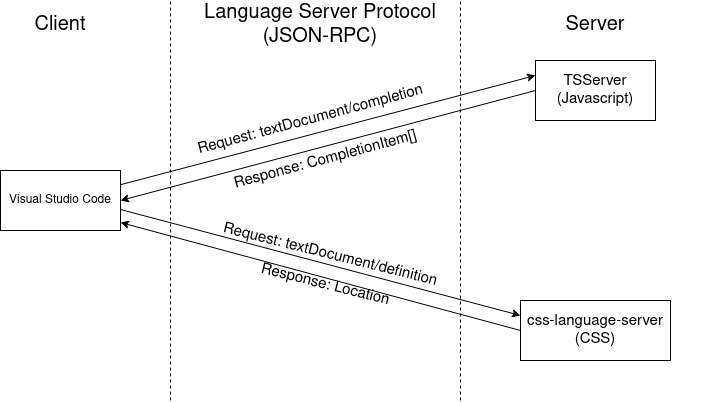
\includegraphics[width=\textwidth]{images/lspcommunication.png}
	\caption{Example client-server interaction using LSP}
	\label{fig:lspcommunication}
\end{figure}


\section{The way forward}

This thesis will present and evaluate a modern tool which provides clone management
capabilities in a real-time IDE environment. The main goal will be to create a tool which
fits well into the development cycle and works in a real-time IDE environment. Areas of
focus will therefore be:

\begin{itemize}
	\item Real-time detection and management of code clones
	\item Code clone refactoring and detection of refactoring-oriented clones
	\item IDE tooling and IDE agnostic tooling like LSP.
	\item Clone ranking, which clones are allowed to stay?
\end{itemize}

\subsection{LSP for IDE-based clone management}

The tool will give programmers the ability to manage clones in their IDE. We will utilize
many feature of LSP, especially code-actions, in order to provide functionality for clone
management to any editor which implements LSP.

The interaction with the LSP server is modelled as user stories as follows:

\begin{itemize}
	\item A programmer wants to see code clones for a single file, the
	      programmer opens the file in their IDE and is displayed diagnostics in the code
	      wherever there are detected clones.

	\item A programmer wants to see all code clones for the current project. The
	      programmer opens the IDE's diagnostic view and will see all code clones detected
	      as diagnostics there. The diagnostic will contain information like where the clone
	      exists, and percentage of duplicated code.

	\item A programmer wants to jump to the corresponding match of a code clone in their
	      editor. The programmer moves their cursor to the code clone diagnostic, invokes a
	      request to see code actions, and invokes the ``Jump to matching clone`` code
	      action. This moves the cursor to the relevant file with the matching code clone
	      selected.

	\item A programmer wants to merge a code clone pair. The programmer moves their cursor
	      to one of the code clones, invokes a request to see code actions, and invokes one
	      of the ``Merge code clone with strategy x`` actions. The strategies presented to
	      the user is dependent on the context of the code clone pair, the programmer will
	      only see the useful / realizable merging strategies.
\end{itemize}

\subsection{Architecture of tool}

Figure \ref{fig:architecture} shows the architecture of the tool. The server communicates
with the IDE and delegates the work of managing clones to the detection engine and the
merge engine. The tool also stores an index of all source code files in the current project.

\subsection{Exploring clone management techniques}

During development of the tool, different techniques for detecting and merging clones will
be explored. The goal will be to find a fitting technique for both detecting and merging
clones in a real-time IDE environment. 

Detection techniques explored will include:

\begin{itemize}
	\item A modified version of Zibran et al. hybrid algorithm\cite{Zibran_real_time_search}
    \item AST-based technique with incremental parsing. Using Tree-sitter, a generator of
        incremental parsers\cite{treesitter}.
    \item More techniques ...
\end{itemize}

Merging tehcniques explored will include:

\begin{itemize}
    \item Refactoring-oriented clone merging\cite{RefactoringOrientedClonesAndMerging}
\end{itemize}

\begin{figure}
	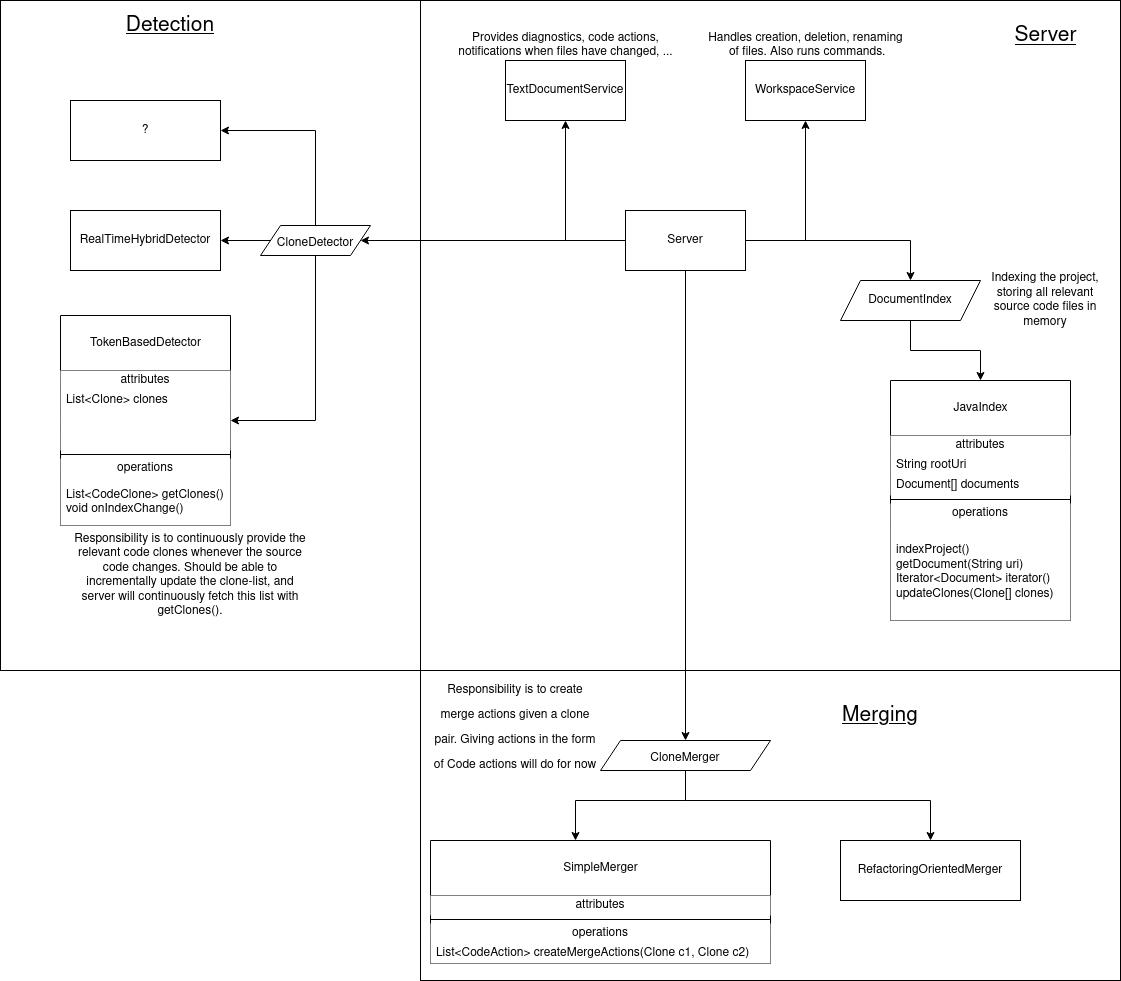
\includegraphics[width=\textwidth]{images/ToolArchitecture.png}
	\caption{Tool architecture}
	\label{fig:architecture}
\end{figure}

The tool will be modular in how techniques are applied for clone management. This
means that the tool will be capable of plugging in different detection engines, merging
engines and file indices. This will be used extensively in our research in order to test
multiple techniques for detection and merging.

\subsection{Evaluation}

We will evaluate this tool based on different criteria, which together will provide a
basis for evaluating the tool as a whole.

\subsubsection{Performance}

Since the tool is focused on efficient detection and management of code clones, real-time
performance of the tool will be a big priority in its evaluation. The tool will implement
different techniques of detecting and merging clones. These will be empirically compared
against each other. The tool will also be evaluated against existing tools empirically.

\subsubsection{Effectiveness in managing clones}

The tool will also be evaluated based on its effectiveness in managing clones. Can we
determine if this tool is better than existing tools at managing or eliminating clones in
the software development cycle?

\subsubsection{Using LSP for refactoring and clone management}

Finally, we will evaluate if LSP is a suitable tool for use in clone management and
refactoring in general. Can LSP provide all the features one would want in a modern clone
management tool? What is missing, and how could the LSP protocol be extended in order to
facilitate this? We believe that if LSP is an appropriate tool to use for clone
management, LSP will also be an appropriate tool for refactoring tools in general.


\newpage
\bibliography{refs}
\bibliographystyle{plain}

\end{document}
